\documentclass[11pt]{article}
\usepackage[utf8]{inputenc}
\usepackage[english]{babel}
%\usepackage{fancyhdr}
%\usepackage{dsfont} %eins als neutrales element
%\renewcommand{\rmdefault}{ppl}
%\usepackage{caption,chngcntr}
%!TeX spellcheck = en_US 
\usepackage{libertine}

\usepackage{hyperref}
\usepackage{mathrsfs}
\usepackage{enumitem} 
\usepackage{paralist}
\usepackage[ 
left=2.5cm,    
right=2.5cm,
top=2cm,
bottom=2cm,
]{geometry}

\usepackage[labelfont={},font={footnotesize}]{caption}

\renewcommand{\figurename}{Fig.}
\renewcommand{\tablename}{Tab.}

%\numberwithin{table}{section}
%\numberwithin{figure}{section}
%\numberwithin{equation}{section}

\usepackage{array}
\newcolumntype{L}[1]{>{\raggedright\let\newline\\\arraybackslash\hspace{0pt}}m{#1}}
\newcolumntype{C}[1]{>{\centering\let\newline\\\arraybackslash\hspace{0pt}}m{#1}}
\newcolumntype{R}[1]{>{\raggedleft\let\newline\\\arraybackslash\hspace{0pt}}m{#1}}

\usepackage{fancybox} 
\usepackage[T1]{fontenc} 

\usepackage[arrow, matrix, curve]{xy}
\usepackage{amsthm}
\usepackage{paralist}
%\usepackage{graphicx} 
%\usepackage{tabularx}
\usepackage{amssymb}
\usepackage{amsmath}


\usepackage{setspace}	
\setstretch{1.2}
\usepackage{natbib}
\bibliographystyle{apalike}

%tikz
\usepackage{tikz}
\usetikzlibrary{shapes.geometric, arrows}
\usetikzlibrary{arrows, arrows.meta, calc, positioning, quotes, shapes}
\usetikzlibrary{automata,positioning}
\usetikzlibrary{positioning, arrows}
\usetikzlibrary{decorations.pathmorphing}
\usetikzlibrary{calc}
\usetikzlibrary{matrix}


\usepackage{float}
\setlength{\parindent}{0pt} 

\definecolor{madrid}{rgb}{0.2,0.2,0.8}
\definecolor{darkgreen}{rgb}{0.2,0.6,0.2}
\definecolor{darkred}{rgb}{0.8,0.2,0.4}
\definecolor{orange}{rgb}{0.9,0.4,0.0}

%\theoremstyle{definition}
%\newtheorem{theorem}{Theorem}
%\newtheorem{definition}{Definition}
%\usepackage{varioref}


\begin{document}
	\huge{ \textbf{Stochastic models to describe turbulent mixing in stably stratified boundary layers} }\\
		\normalsize
		
		
%	\section{Overview Paper}
%	recommended papers: \\
%	\textbf{\cite{Mahrt2014}}: Review Paper, nice explanations, comparison of vertical structure of weakly and strongly SBLs, Layer of BL, BL regimes, turbulence in very stable regimes, other influences: submeso, waves, ... \\
%	\textbf{\citet{Sandu2013}}: Problems of NWPs in predicting SBLs (depth overestimated, LLJ too weak), turbulent diffusion parametrization in ECMWF (K parametrization), Comparison to UKMO and GFS, Result: less diffusive turbulence scheme $\rightarrow$ improves representation of SBL winds (LLJ) + deepening of lows/stronger highs, but: also detrimental influences (large-scale flows, temperature 2m), other possibilities for adjusting: orography drag parametrization, land-atmosphere-coupling \\
%	\textbf{\citet{Mahrt2020}}: Non-stationary boundary layers, non-stationarity due to thermal forcing/ dynamical forcing/clouds, spectral gap only in stationary case, Eulerian and Lagrangian stability, quasi-equilibrium and non-equilibrium turbulence \\
%	\textbf{\citet{Kral2021}}: investigating SBL with remote sensing and different unmanned aircraft systems (UAS), case studies \\
%	
%	stochastic modeling \\
%	\textbf{\cite{Vercauteren2015}}: method FEM-VARX (notes below) \\
%	\textbf{\cite{BoykoDiss2022}}: Dissertation, methods FEM-VARX and FEM-H$^1$-SDE (notes below)  \\
%	\textbf{\cite{BoykoPaper2022}}: preprint, method FEM-H$^1$-SDE (notes below) \\
%	
%	others to SBL: \\
%	\textbf{\citet{AnsorgeDiss2016}}: Dissertation, detailed description of SBL regimes in Introduction\\
%	\textbf{\citet{Stiperski2018,Stiperski2019}}: Extend MOST for anisotropy and heterogeneous surfaces\\ 
%	
%	general: \\
%	\textbf{\citet{Li2012}}: ratio of $\phi_H, \phi_m$, Prandtl number  \\
%	\textbf{\citet{Calaf2022}}: overview modelling approaches in NWPs, triple decomposition
%	
	\section{Planetary Boundary Layer -- Theory}
		
		Basic equations: \\
		To describe vertical diffusion by turbulent motion: we have to select conserved quantities under adiabatic processes
		\begin{figure}[H]
			\small
			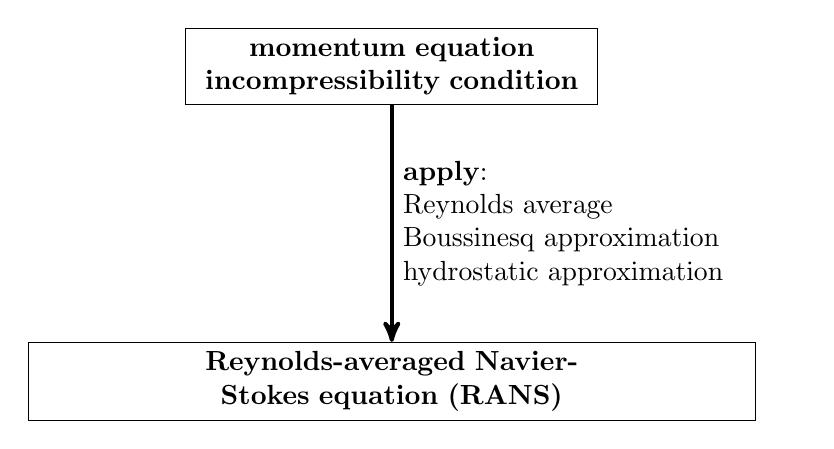
\begin{tikzpicture}
				\node(start)  [draw, text width = 5cm,align=center] at (0,0)  {\textbf{momentum equation\\incompressibility condition}};
				
				\node(rans)  [draw, text width = 9cm,align=center] at (0,-4)  {\textbf{Reynolds-averaged Navier-Stokes equation (RANS)}};
				%\node(ranseq)  [text width = 5cm,align=center] at (0,-5)  {$$\frac{\partial \overline{\boldsymbol{v}}}{\partial t} + \overline{\boldsymbol{v}}\cdot\nabla \overline{\boldsymbol{v}} - f \boldsymbol{k}\times\overline{\boldsymbol{v}} = -\frac{1}{\rho_0} \nabla p + \nu \nabla^2\overline{\boldsymbol{v}} $$};
				
				\draw[->, >=stealth',line width=1.5pt,text width=5cm, align=left] (start) -- (rans) node[midway,right] {\textbf{apply}: \\Reynolds average \\ Boussinesq approximation\\hydrostatic approximation} ;	
				
			\end{tikzpicture}
			\centering
			\caption{}
		\end{figure}
		
		(to be continued) \\
		
		
	\section{Planetary Boundary Layer -- Modelling}
	Why we need a realistic representation of the PBL:
	\begin{compactenum}
		\item[-] PBL parametrization determines together with the surface parametrization the surface fluxes and redistributes them in the PBL $\rightarrow$ they introduce the diurnal pattern in the surface field
		\item[-] PBL processes are relatively quick $\rightarrow$ PBL responds to its forcing within a few hours $\rightarrow$ PBL is always in a quasi-equilibrium with large-scale forcing
		\item[-] large-scale budgets of momentum, heat and moisture are considerably affected by the surface fluxes
		\item[-] model variables in the PBL are important model output
		\item[-] PBL interacts with other processes, e.g. cloud formation
	\end{compactenum}
	
	\begin{figure}[H]
		\small
		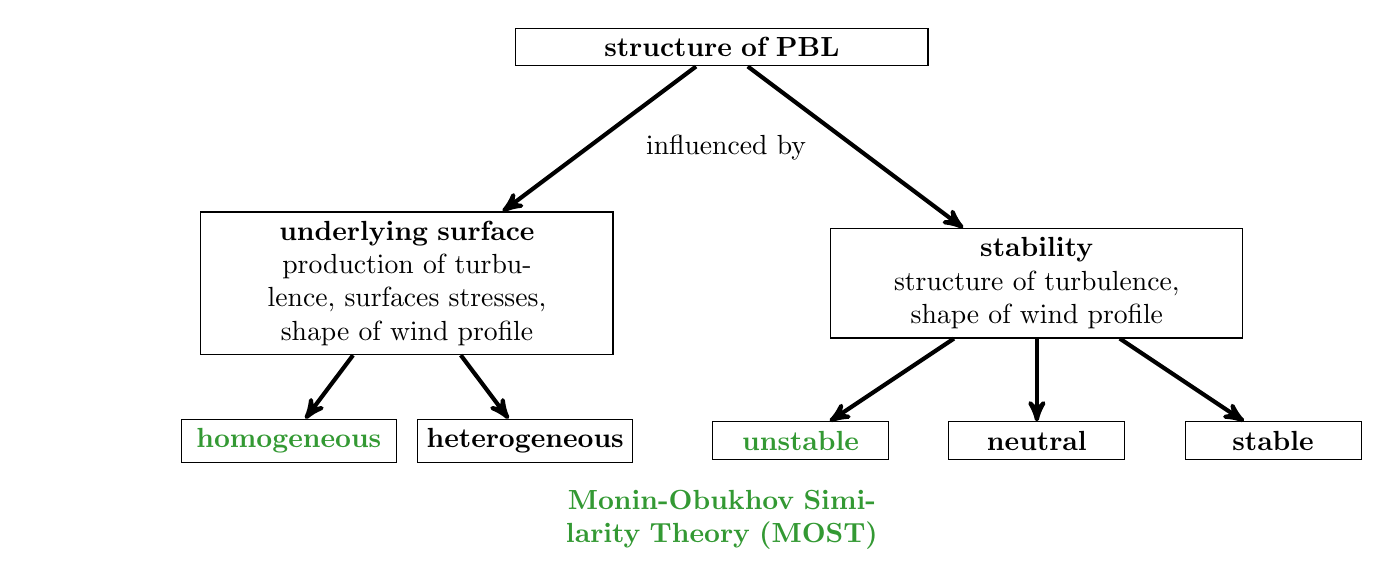
\begin{tikzpicture}
		\node(str)  [draw, text width = 5cm,align=center] at (0,0)  {\textbf{structure of PBL}};
		\node(surface)  [draw, text width = 5cm,align=center] at (-4,-3)  {\textbf{underlying surface}\\production of turbulence, surfaces stresses, shape of wind profile};
		\node(stability)  [draw, text width = 5cm,align=center] at (4,-3)  {\textbf{stability}\\structure of turbulence, shape of wind profile};

		\node(unstable)  [draw, text width = 2cm,align=center] at (1,-5)  {\textcolor{darkgreen}{\textbf{unstable}}};
		\node(neutral)  [draw, text width = 2cm,align=center] at (4,-5)  {\textbf{neutral}};
		\node(stable)  [draw, text width = 2cm,align=center] at (7,-5)  {\textbf{stable}};
		
		\node(hom)  [draw, text width = 2.5cm,align=center] at (-5.5,-5)  {\textcolor{darkgreen}{\textbf{homogeneous}}};
		\node(het)  [draw, text width = 2.5cm,align=center] at (-2.5,-5)  {\textbf{heterogeneous}};
		
		\node(most)  [text width = 7cm,align=center] at (0,-6)  {\textcolor{darkgreen}{\textbf{Monin-Obukhov Similarity Theory (MOST)}}};
		
		%\draw[->, >=stealth',dashed,line width=1.5pt,text width=2cm, align=left] (sse) -- (model) node[midway,left] {} ;			
		\draw[->, >=stealth',line width=1.5pt,text width=7cm, align=right] (str) -- (surface) node[midway,left] {} ;
		\draw[->, >=stealth',line width=1.5pt,text width=3cm, align=center] (str) -- (stability) node[midway,left] {influenced by} ;	
		
		\draw[->, >=stealth',line width=1.5pt,text width=3cm, align=center] (surface) -- (hom) node[midway,left] {} ;	
		\draw[->, >=stealth',line width=1.5pt,text width=3cm, align=center] (surface) -- (het) node[midway,left] {} ;	
		
		\draw[->, >=stealth',line width=1.5pt,text width=3cm, align=center] (stability) -- (stable) node[midway,left] {} ;	
		\draw[->, >=stealth',line width=1.5pt,text width=3cm, align=center] (stability) -- (unstable) node[midway,left] {} ;	
		\draw[->, >=stealth',line width=1.5pt,text width=3cm, align=center] (stability) -- (neutral) node[midway,left] {} ;	
		
		\end{tikzpicture}
		\centering
		\caption{}
	\end{figure}

	\subsection{Diurnal Pattern}
	Diurnal pattern (only over land): \\
	unstable (convective) BL: during daylight $\rightarrow$ enhanced turbulent mixing $\rightarrow$ profiles of meteorological quantities are more uniform (near surface: super-adiabatic, then approximately uniform, then capped inversion); fluxes:heat flux into the ground, sensible heat flux into the atmosphere and latent heat of evaporation \\
	stable BL: inversion layer \\
	(Fig!)
	
	
	\subsection{Surface Heterogeneity}
	$\ell_h$: length scale of surface thermal heterogeneity (thermal patch size)\\
	$\ell_d$: length scale of the mean vertical dynamics \\
	
	ratio of the length scales:
	\begin{align}
		\ell_d \begin{cases}
			\ll \ell_h & \rightarrow \textrm{vertical motions are blended, e.g., strong geostrophic forcing} \\
			\ge \ell_h & \rightarrow \textrm{active interaction, so called (turbulence organized structures, TOS)}
		\end{cases}	
	\end{align}
 it depends whether $\ell_h$ is larger or smaller (need for parametrization) than the model resolution \\
 
 definition of thermal heterogeneity parameter $\mathcal{H}$ \citep{Margairaz2020a} (their Fig. 2 is a nice explanation):
 \begin{align}
 	\mathcal{H} := \frac{\ell_d}{\ell_h} \sim \frac{g \ell_h}{U_g^2} \frac{\Delta T}{\overline{T}}
 	\begin{cases}
 		\gg 1 & \rightarrow \textrm{heterogeneity dominates flow dynamics (TDFs important)} 	\\
 		\ll 1 & \rightarrow \textrm{shear dominates (TDFs negligible)}
 	\end{cases}
 \end{align}
rewrite: first term (inverse squared Froude number) and second term (relative measure of the surface-temperature heterogeneity, i.e. upper limit on the buoyancy term) \\

Dispersive fluxes: arise when a time-averaged variable is represented as the sum of a time- and spatially-averaged variable (new covariances arise)\\ 
 
 
	\subsection{Similarity Theory}
	problem: turbulence is too complicated to enable a derivation of parametrizations from first principles $\rightarrow$ empirical relationships based on observations $\rightarrow$ similarity theory provides the framework to organize and group the experimental data \\

			\begin{figure}[H]
		\small
		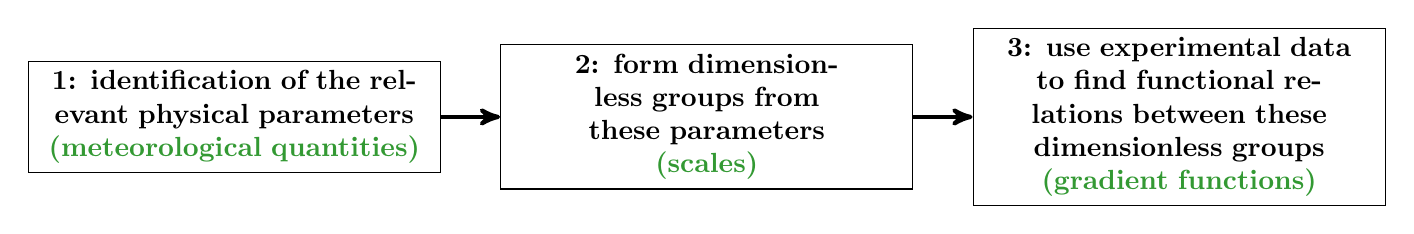
\begin{tikzpicture}
		\node(most1)  [draw, text width = 5cm,align=center] at (0,0)  {\textbf{1: identification of the relevant physical parameters\\\textcolor{darkgreen}{(meteorological quantities)}}};
		\node(most2)  [draw, text width = 5cm,align=center] at (6,0)  {\textbf{2: form dimensionless groups from these parameters \\\textcolor{darkgreen}{(scales)}}};
		\node(most3)  [draw, text width = 5cm,align=center] at (12,0)  {\textbf{3: use experimental data to find functional relations between these dimensionless groups\\\textcolor{darkgreen}{(gradient functions)}}};
		
		\draw[->, >=stealth',line width=1.5pt,text width=5cm, align=left] (most1) -- (most2) node[midway,right] {} ;
		\draw[->, >=stealth',line width=1.5pt,text width=5cm, align=left] (most2) -- (most3) node[midway,right] {} ;
		\end{tikzpicture}
		\centering
		\caption{General approach in similarity theory.}
	\end{figure}
		\textcolor{darkgreen}{gradient functions:} direct expressions for exchange coefficients as they relate fluxes to gradients \\
		consider different parts of PBL (surface layer and outer layer) and different limiting cases (e.g., stability) \\
		
	method: Buckingham Pi dimensional analysis \\
	
	\textbf{Surface Layer}
	\begin{compactenum}
		\item[-] shallow fraction of the PBL near the surface where the fluxes are approximately equal to the surface values $\rightarrow$ constant flux layer
		\item[-] $z/h \ll 1$
		\item[-] relevant parameters for the wind profiles: momentum flux, buoyancy flux, height above the surface
		\item[-] relevant scales: friction velocity, Obukhov length, turbulent potential temperature scale, turbulent humidity scale
		\item[-] surface layer has two relevant length scales $z, L \rightarrow$ write all dimensionless quantities as function of $z/L$
		\item[-] dimensionless gradients, e.g. $\Phi_m(z(L)$) 
		\item[-] limiting cases
		\begin{align}
			\frac{z}{L} \begin{cases}
			= 0 &\rightarrow \textrm{neutral limit} \\
			\ll-1 &\rightarrow \textrm{free convective limit}
			\end{cases}
		\end{align} 
		neutral limit: Obukhov length drops out as a relevant scale $\rightarrow$ dimensionless wind gradient has to be constant \\
		convective limit: large values of $-z/L$ imply that the production of turbulence by bouyancy is much larger than the production by wind shear $\rightarrow$ friction velocity is irrelevant as scaling quantity\\
	\end{compactenum}
	
	\textbf{Outer Layer}
	\begin{compactenum}
		\item[-] fluxes are not constant, but decrease monotonically from their surface values to small values at BL top
		\item[-] if BL height ($h$) is not determined externally (e.g. capped inversion), but by BL processes, then the BL height must be proportional to $u_*/f$
		\item[-] cases: neutral, unstable, stable
	\end{compactenum}

	\begin{tabular}{llll}
	&	\textbf{neutral} & \textbf{unstable} & \textbf{stable} \\
	\hline 
	relevant parameter &$u_*, F, z$ & $(\overline{w'\theta'}_0), h,z$ & $\tau/\rho, \overline{q'\theta'}, g/\theta$\\	
	&&&$\rightarrow$ define \textit{local} Obukhov length $\Lambda$ \\
	&&&$\rightarrow$ functions of $z/\Lambda$ \\
	omit &&$u_*$& $u_*$ \textit{cannot} be omitted (friction is\\
	&&& only source of turb. production) \\
	scales &&$w_*. \theta_*$& \\
	&&well-mixed \\
	&&$\rightarrow$ profiles nearly uniform
\end{tabular}
	
	remarks to stable: To limit the number of independent parameters Nieuwstadt (1984) introduced the idea of local scaling $\rightarrow$ explanation: in SBL turbulence is generated by shear and destroyed by buoyancy and viscous dissipation: bouyancy acts vertically $\rightarrow$tends to limit the vertical extent over which mixing takes place $\rightarrow$ limits turbulent length scale\\
	decoupling of turbulence from the surface $\rightarrow$ local fluxes might be more suitable as direct scaling parameters \\
	%TODO compare obukohov length and local obukhov length
	
	large $z/\Lambda \rightarrow$ turbulence length is $\Lambda$, surface has no influence $\rightarrow$ $z$ should drop out of scaling relations $\rightarrow$ gradient functions become linear in $z/\Lambda$ (z-less scaling) -> Fig 13\\
	
	\textbf{Surface Boundary Conditions}
	\begin{compactenum}
		\item[-] PBL parametrization introduces need for BC at the surface: vanishing velocity, specified temperature and humidity (LSP)
		\item[-] additional problem arises: BCs are connected to the surface roughness length (=integration constant in the logarithmic wind profile, related to small scale surface inhomogeneities that determine the surface drag) $\rightarrow$ pressure forces on the roughness elements transfer wind stress to the surface (form drag) $\rightarrow$ form drag has no equivalent for scalar quantities $\rightarrow$ roughness length for momentum, heat and moisture are generally different
		\item[-] roughness length is a surface characteristic and related to its geometry $\rightarrow$ but only way to determine it is via wind profile $\rightarrow$ measuring (e.g, land-use maps)
		\item[-] in models: effective roughness length (account for all the terrain inhomogeneities in the box)
		\item[-] roughness length over sea
	\end{compactenum}
	
	\subsection{PBL Schemes for PBL}
	(notes mainly based on \citep{ECMWF2002}) \\
	
	\textbf{Geostrophic transfer laws}
	\begin{compactenum}
		\item[-] application: for models that have no model levels in the PBL
		\item[-] based on: boundary layer similarity for the steady state PBL
		\item[-] assumption: lowest level is at the top or above the PBL
		\item[-] bulk transfer laws: express surface fluxes with model variables above the PBL (geostrophic) \\
		eqs
		\item[-] pros: very simple, firs order approximation
		\item[-] cons: no diurnal cycle, no effects of stability, no forecast products in PBL physics poorly represented
		\item[-] extension: introduce stability effects in transfer coefficients \\
	\end{compactenum}

	\textbf{Integral models (slab, bulk models)} 
	\begin{compactenum}
		\item[-] idea: entire PBL is characterized by a limited number of parameters $\rightarrow$ prognostic equations are derived for them
		\item[-] assumption: similarity form (eq 81) exists
		\item[-]
		\item[-] pros: relatively simple, PBL does not have to be resolved by vertical layer structure of the model, physically realistic for mixed layer
		\item[-] cons: difficult to implement (moving PBL height), similarity profiles for SBL are complicated/unknown, difficult to handle regime transitions \\
	\end{compactenum}

	\textbf{Grid point models with K-closure} 
	\begin{compactenum}
		\item[-] application: models that resolve PBL explicitly
		\item[-] idea: analogy to molecular diffusion \\ (eqs 88, 89) $\rightarrow$ surface layer similarity provides the formulation of K near the surface \\
		implicit to explicit closure:  substitute Obukhov length $\rightarrow$ gradient Richardson number
		\begin{align}
			Ri = \frac{g}{\theta_v} \frac{\frac{d\theta_v}{dz}}{\vert \frac{d \boldsymbol{u}}{dz} \vert^2} = \frac{l}{kL} \frac{\Phi_H}{\Phi_m^2}	
		\end{align} 
		\item[-] much more efficient to specify stability functions that depend on Ri number because then we have the fluxes explicitly in terms of model variables $\rightarrow$ derived from observations
		\item[-] main difficulty: specification of stability functions
		\item[-] pros: fully consistent with the grid point formulation of the model, the same scheme can be used for stable, neutral, unstable, land, sea; very realistic for SBL if sufficient resolution
		\item[-] cons: a number of levels is needed to resolve the PBL, limitations in the concept of local diffusion (shape of stability functions is subject to ongoing debate), problems in intermittent regime, discretization errors especially in shallow PBL, does not account for integral aspects, physics of convective PBL is not adequately described, does not describe counter-gradient fluxes \\
	\end{compactenum}	

	\textbf{K-profile closure}
	\begin{compactenum}
		\item[-] application: low resolution models
		\item[-] idea: express exchange coefficients not in local gradients but as integral profiles for the entire PBL
		\item[-] scaling parameters: PBL height, surface fluxes
		\item[-] formulation \\
			eqs 114-119 \\
			implicit $\rightarrow$ explicit 
		\item[-] pros: extremely robust to numerical stability, non-local aspects allow for description of entrainment
		\item[-] cons: difficult to develop generalizations for cloudy or baroclinic environments \\
	\end{compactenum}
	
	\textbf{TKE-closure} 
	\begin{compactenum}
		\item[-] idea: simplest higher order closure by specification of the diffusion coefficients with a prognostic variable for the TKE 
		\item[-] formulation eqs 126 ...\\
		using TKE equation to have a prognostic equation for the turbulent velocity scale, diagnostic one is still needed for the length scales 
		\item[-] pros: simplest closure with some non-local aspects of turbulence; enables the introduction of more advanced cloud schemes
		\item[-] cons: demanding on vertical resolution, in general: higher-order closure schemes do not necessarily reproduce surface layer similarity $\rightarrow$ may result in inconsistency between the lowest model level and the layers aloft
	\end{compactenum}
	
	\subsection{Modelling stable PBL}
	Why SBL is more difficult to understand then CBL \citep{LeMone2019}:
	\begin{compactenum}
		\item[-] smaller scale (smaller PBL height $\rightarrow$ smaller vortices)
		\item[-] weaker turbulence
		\item[-] greater sensitivity to terrain (i.e., abrupt change in surface characteristics $\rightarrow$ BL out of equilibrium $\rightarrow$ circulation will develop) $\rightarrow$ more difficult to observe
	\end{compactenum}
	
	
	
	
	
	\subsection{Multiresolution decomposition}
	features of MRD that are not inherent in the Fourier decomposition according to \citet{Howell1997}:
	\begin{compactenum}
		\item[-] the peak in multiresolution cospectra depends
		mostly on the width of the dominant (local) flux events whereas the wavelength
		of the peak in Fourier cospectra depends on the principal periodicity
		\item[-] Each mode of the multiresolution decomposition corresponds to a simple unweighted (nonoverlapping) moving average and thus, satisfies the rules of
		Reynolds averaging.
		\item[-] N arithmetic operations (compared to N log(N) for FFT)
		\item[-] Each mode of the multiresolution decomposition corresponds to a simple unweighted (nonoverlapping) moving average and thus, satisfies the rules of
		Reynolds averaging.
	\end{compactenum}
	
	
	
	\begin{figure}[H]
		\small
		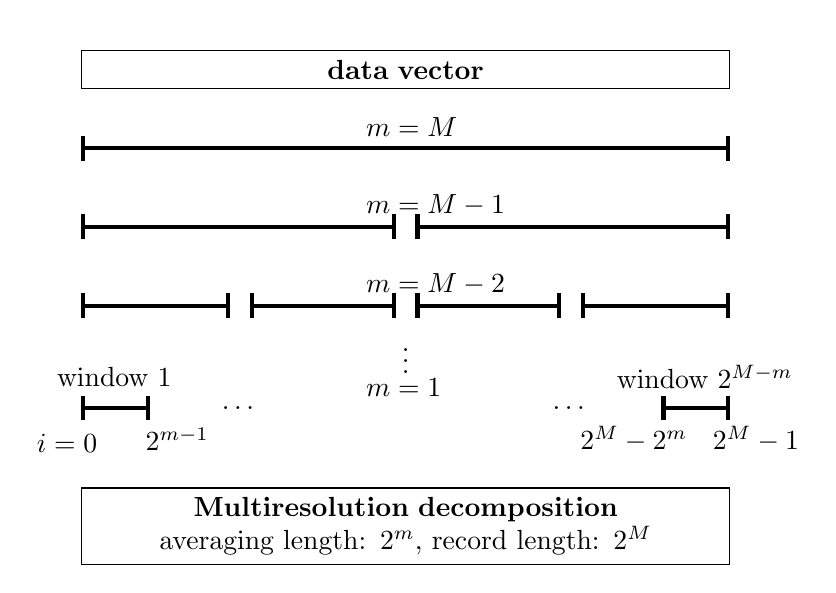
\begin{tikzpicture}
			\node(start)  [draw, text width = 8cm,align=center] at (0,0)  {\textbf{data vector}};
			\node(mrd)  [draw, text width = 8cm,align=center] at (0,-5.8)  {\textbf{Multiresolution decomposition} \\
			averaging length: $2^{m}$, record length: $2^{M}$};
			\node(h1) at (-4.25,0)  {};
			\node(h2) at (4.25,0)  {};
			\node(h3) at (0,0)  {};
			\node(h4) at (-2.1,0)  {};
			\node(h5) at (2.1,0)  {};
			\node(h6) at (-3.125,0)  {};
			\node(h7) at (3.125,0)  {};
			\node(dots) at (0,-3.6)  {$\vdots$};
			\node(dots2) at (-2.1,-4.3)  {$\dots$};
			\node(dots3) at (2.1,-4.3)  {$\dots$};
			\draw[|-|,line width=1.5pt,text width=5cm, align=left,transform canvas={yshift=-10mm}] (h1) -- (h2) node [above] at (2,0) {$m=M$} ;
			\draw[|-|,line width=1.5pt,text width=5cm, align=left,transform canvas={yshift=-20mm}] (h1) -- (h3) node [above] at (2,0) {$m=M-1$} ;
			\draw[|-|,line width=1.5pt,text width=5cm, align=left,transform canvas={yshift=-20mm}] (h2) -- (h3);
			
			\draw[|-|,line width=1.5pt,text width=5cm, align=left,transform canvas={yshift=-30mm}] (h1) -- (h4)
			node [above] at (2,0) {$m=M-2$};
			\draw[|-|,line width=1.5pt,text width=5cm, align=left,transform canvas={yshift=-30mm}] (h3) -- (h4);
			\draw[|-|,line width=1.5pt,text width=5cm, align=left,transform canvas={yshift=-30mm}] (h3) -- (h5);
			\draw[|-|,line width=1.5pt,text width=5cm, align=left,transform canvas={yshift=-30mm}] (h2) -- (h5);
			
			\draw[|-|,line width=1.5pt,text width=5cm, align=left,transform canvas={yshift=-43mm}] (h1) -- (h6)
			node [above] at (2,0) {$m=1$};
			\draw[|-|,line width=1.5pt,text width=5cm, align=left,transform canvas={yshift=-43mm}] (h2) -- (h7);
			
			
			\node(i0) at (-4.3,-4.75)  {$i=0$};
			\node(i1) at (-2.9,-4.7)  {$2^{m-1}$};
			\node(i2) at (2.9,-4.7)  {$2^{M}-2^{m}$};
			\node(im) at (4.45,-4.7)  {$2^{M}-1$};
			\node(w1) at (-3.7,-3.9)  {window 1};
			\node(wm) at (3.8,-3.9)  {window $2^{M-m}$};
		\end{tikzpicture}
		\centering
		\caption{Schematic visualization of the multiresolution decomposition procedure according to \citet{Howell1997}.}
	\end{figure}
	
	
	
	\section{Relevance: Link to climate models}
	\citet{Davy2014}:
	\begin{compactenum}
		\item[-] surface air temperature has become one of the most
commonly-used metrics to assess our climate
		\item[-] The magnitude of the surface air
temperature response to forcing is determined by three components: the magnitude of the forcing, any feedback processes
involved, and the effective heat capacity of the system
		\item[-] The effective heat capacity of the atmosphere is defined by
the region of turbulent mixing through which the heat is
mixed i.e. it is defined by the depth of the ABL
		\item[-] mathematical description through Energy-Budget-Model 
		\begin{align}
			\frac{d\theta}{dt} = \frac{Q}{\rho c_p h} 
		\end{align}
		Q: heat flux divergence within the ABL \\
		h: depth of ABL
		
		
	\end{compactenum}
	
	
	\section{Stochastic Models}
	
	\subsection{Why using stochastic models?}
	\citet{Palmer2019}: ''any computational representation of climate should be
	partially stochastic'', because:
	\begin{compactenum}
		\item[a)] nature of symmetries of the underlying equations
		\item[b)] improved forecast reliability of stochastic models (inherent variability)
		\item[c)] algorithmic efficiency\\
	\end{compactenum}	
	
	historically: unresolved processes are represented by semi-empirical formulas (''parametrizations'') $\rightarrow$ deterministic models estimate the bulk effect of the subgrid-scale processes on the grid-scale flow (small scales are treated as 'slaves' to the large scale), assumptions:
	\begin{compactenum}
		\item[-] the subgrid processes are in local quasi-equilibrium
		\item[-] scale separation between resolved and unresolved flow\\
	\end{compactenum}
	
	advantages of stochastic parametrizations:
	\begin{compactenum}
		\item[-] applicable in the grey-zone
		\item[-] stochasticity can cascade from small to large timescales
		\item[-] transience
		\item[-] simulation of quasi-stationary weather regimes
		\item[-] allows for low-precision modelling
		\\
	\end{compactenum}

	stochastic parametrizations should take into account:
	\begin{compactenum}
		\item[-] conservation laws
		\item[-] must avoid breaking the holistic balance to much
		\item[-] developed ab inito stochastically
		\item[-] testing SPs: coarse graining
	\end{compactenum}
	e.g.: symmetry properties of Navier-Stokes equation: scaling symmetry $\rightarrow$ self-similar nature of fluid turbulence $\rightarrow$ consisten with the ubiquitos existence of power-law behaviour\\
	
	more theoretical approach to stochastic parametrizations: Mori-Zwanziger projector operator theory
	
	\subsection{Stochastic Differential Equations (SDEs)}
	(nice intro by \citet{Sarkka2014}) \\
	vector differential equation of the form:
	\begin{align}
		\frac{d\boldsymbol{x}}{dt} = \textcolor{madrid}{\boldsymbol{f}(\boldsymbol{x},t)} + \textcolor{orange}{\boldsymbol{L}(\boldsymbol{x},t)}\textcolor{darkred}{\boldsymbol{w}(t)}	
	\end{align}
	$\textcolor{darkred}{\boldsymbol{w}(t)}$: vector of forcing functions $\rightarrow$ can be interpreted as stochastic process (white noise) $\rightarrow$ then: solution is stochastic process\\
	$\textcolor{madrid}{\boldsymbol{f}(\boldsymbol{x},t)}$: nominal dynamics of the system \\
	$\textcolor{orange}{\boldsymbol{L}(\boldsymbol{x},t)}$: dispersion matrix, determines how the noise enters the system \\
	
	rewritten: Itô process (1D)
	\begin{align}
		dx = \underbrace{\mu(x,t)}_{\textrm{drift}} \:dt + \underbrace{\sigma(x,t)}_{\textrm{diffusion}} \: \underbrace{dW}_{\textrm{Wiener ´process}}
	\end{align}
	Remark integrating this equation: we need a different type of integral (not Riemann, Lebesgue, Stieltjes), because integrand and integrator are now stochastic processes
	
	\subsection{Stochastic models for Boundary Layer Meteorology}
	\begin{table}[H]
		\begin{tabular}{lll}
			&\textbf{FEM-VARX} & 	\textbf{FEM-H$^1$-SDE} \\
			\hline
			developed & Horenko, 2010 & Boyko, 2022 \\
			applied & Vercauteren and Klein, 2015 & Boyko, 2022 \\
			\hline
			advantages & + several dimensions & + continuous \\
			&+ memory effect & + model noise \\
			disadvantages & - discrete & - only one dimension \\
			& - noise a posteriori & - no memory effect 
		\end{tabular} 
	\centering
	\end{table}
Assume that the dynamics (Vercauteren and Klein, 2015: time evolution of turbulent mixing) can be described by a stochastic process with external factors $\rightarrow$ \textbf{VARX:}
\begin{align}
	x(t) = \mu(t) + A(t) \cdot \phi_1(x_{t-\tau}, ..., x_{t-m\tau}) + B(t) \cdot \phi_2(u_t, ...,u_{t-p\tau})  + c(t) \epsilon_t
\end{align}

with:\\
$\phi_1(x_{t-\tau}, ..., x_{t-m\tau})$: m previous observations of process x(t) \\
$\phi_2(u_t, ...,u_{t-p\tau})$: external factors, currently (t) and p previously \\
$\epsilon_t$: Gaussian noise\\

\textbf{FEM-VARX}: optimal clustering in several VARX processes\\

\citet{Vercauteren2015}:\\
model vertical velocity fluctuations with streamwise velocity at different scales\\

\citet{BoykoDiss2022}:
\begin{compactenum}
	\item[-] determine memory depth by evaluating the partial cross-correlation function (pacf) between U and $\sigma_w$ (same quantities like Vercauteren and Klein, 2015)
	\item[-] finding appropriate number of clusters: (1) AIC, BIC -- difficult here, (2) recursive application of FEM-VARX
	\item[-] indicator for stability: bulk Richardson number (= discrete version of the normal Ri)
	\item[-] multiresolution decomposition (MRD) $\rightarrow$ identify average turbulent timescale \\
\end{compactenum}

	
	%\newpage
	

\textbf{FEM-H$^1$-SDE} \citep{BoykoDiss2022,BoykoPaper2022} 
	\begin{compactenum}
		\item[-] triple decomposition:
		\begin{align}
			T(\boldsymbol{x},t) = \overline{T}(\boldsymbol{x},t) + \widehat{T}(\boldsymbol{x},t) + T'(\boldsymbol{x},t)
		\end{align}
		interpretation: (here: insert discussion about ensemble mean) \\
		$\overline{T}(\boldsymbol{x},t):$ long-time average (1 h), considered as the timescale at which MOST is valid, meaning that the mean shear is sufficient to maintain Kolmogorov-like turbulence connecting the BL to the ground \\
		$\widehat{T}(\boldsymbol{x},t):$ short-time average (3 Min), includes turbulence but excludes sub-mesoscale motions $\rightarrow$ scale band corresponding to submeso-scale motions is defined between 1h and 3 min (Fig. 1 in \citet{BoykoPaper2022})
		\item[-] based on TKE closure of order 1.5 (Stull, 1988) with kinematic eddy-viscosity coefficient (models the momentum diffusion due to turbulent eddies)
		\begin{align}
			K_m = \alpha \ell_m \sqrt{e}
		\end{align}
	($\alpha$: modelling constant, $\ell_m$: turbulent mixing length for momentum, $e$: TKE), similarly the eddy heat conductivity coefficient $K_h$ should be specified for a complete closure
	\item[-] seek: to model $\ell_m$ in term of local Ri number (assuming constant Prandtl number $Pr = K_m/K_h$)
	\item[-] definition of $\ell_m$:
	\begin{align}
		\ell_m := \frac{\widehat{u_*}}{\partial \overline{U}/\partial z} = \frac{\kappa z}{\phi_f}
	\end{align}
with friction velocity $\widehat{u_*} = (\widehat{u'w'}^2+\widehat{v'w'}^2)^{(1/4)}$, $\kappa:$ von Karman constant, $\phi_f$ momentum stability correction function following MOST determined from the flux-gradient relationship, it scales the amount of turbulent mixing with atmospheric stability, $\overline{U} = \sqrt{\overline{u}^2+\overline{v}^2}$
	\item[-] next $\phi$ will be modelled stochastically
	\begin{align}
		\phi(t) := \frac{\kappa z \vert \partial \overline{U} / \partial z \vert}{\widehat{u_*}}
	\end{align}
	interpretation of the different averaging scales: ''driving hypothesis is that submeso-scale motions induce transient changes in the mixing length due to departure of the turbulence from statistical equilibrium'' (S. 7) $\rightarrow$ to represent the lack of statistical equilibrium, the uncertainty induced by the short-scale deviations in $\phi$ will be modelled with a SDE
	\item[-] parameter estimation with model-inference methodology by \citet{Boyko2021}: this method is of one-dimensional form $\rightarrow$ reason that the scaling function have to be height independent
	\end{compactenum}
	
	\begin{figure}[H]
		\small
		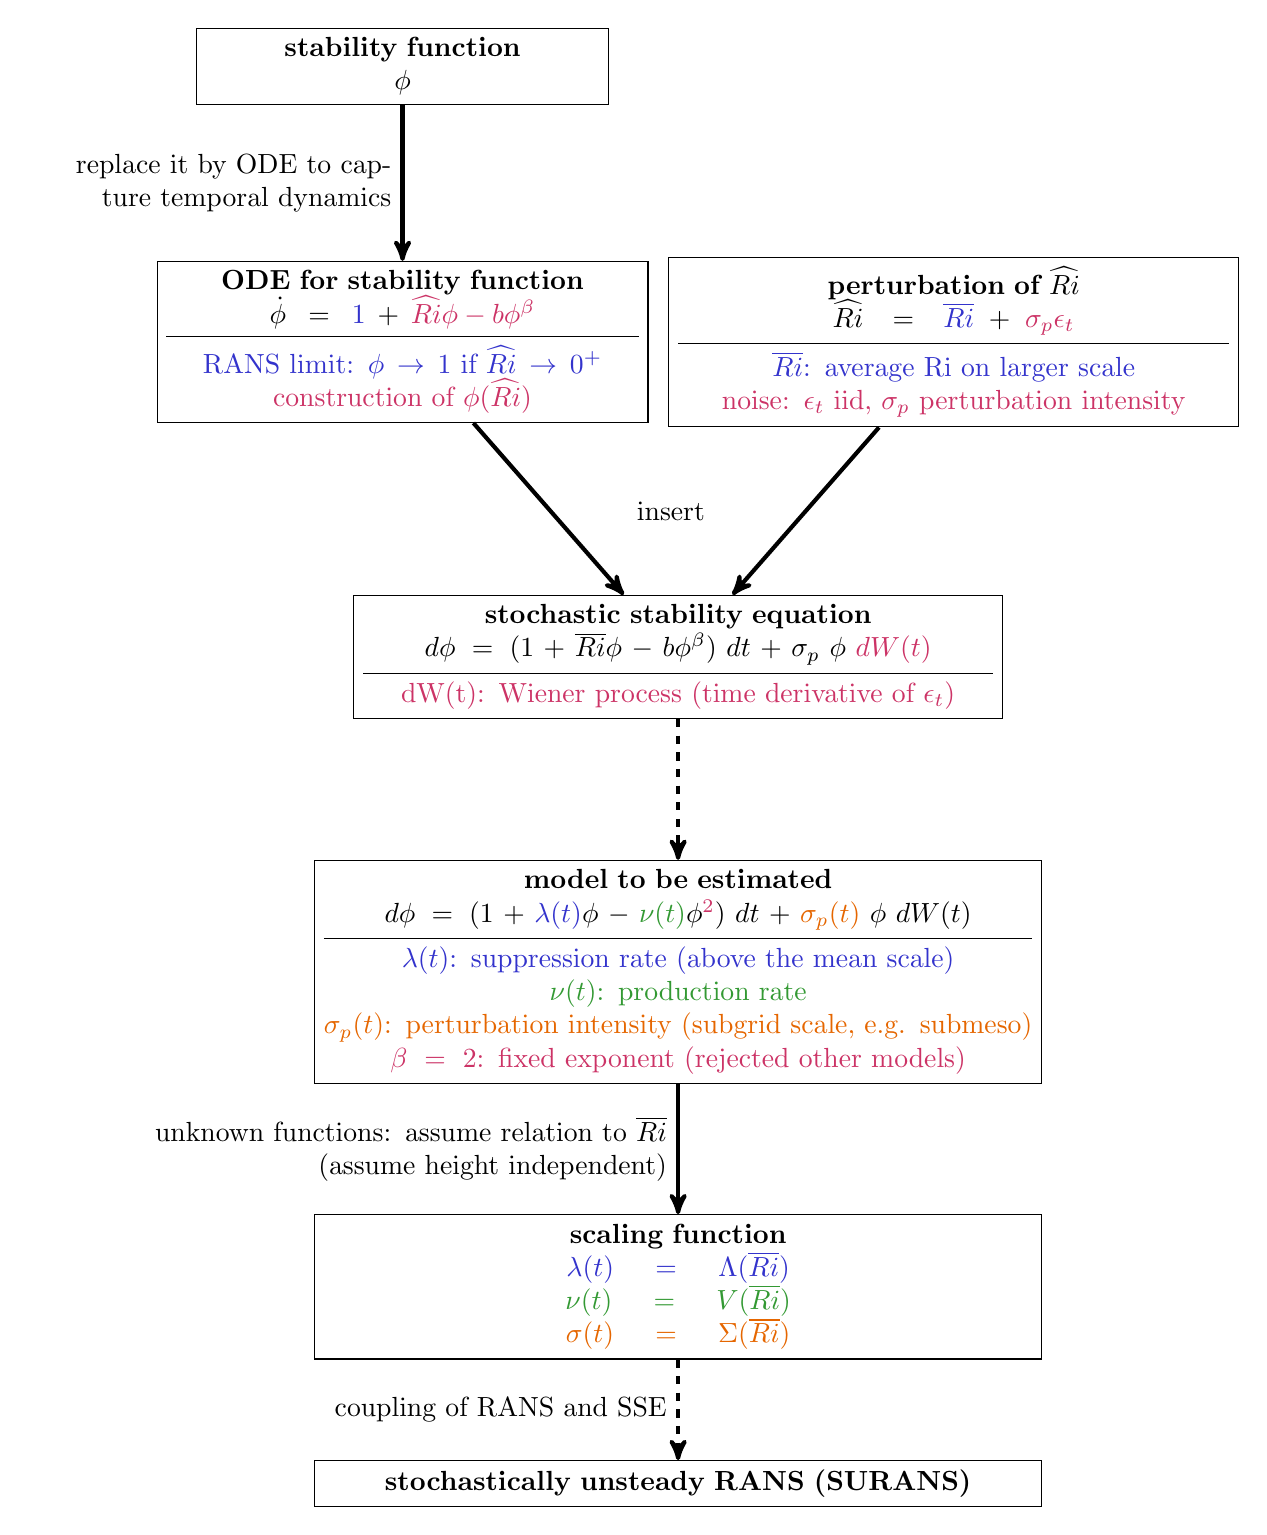
\begin{tikzpicture}
			\node(start)  [draw, text width = 5cm,align=center] at (0,0)  {\textbf{stability function\\ $\phi$}};
			
			\node(ode) [draw,text width=6cm,align=center] at (0,-3.5)  {\textbf{ODE for stability function} \\ 
				$\dot{\phi}=\textcolor{madrid}{1}+\textcolor{darkred}{\widehat{Ri} \phi- b \phi^\beta}$ \\[0.1cm]
				\hrule
				\vspace{0.1cm}
				\textcolor{madrid}{RANS limit: $\phi \rightarrow 1 \textrm{ if } \widehat{Ri}\rightarrow0^+$} \\
				\textcolor{darkred}{construction of $\phi(\widehat{Ri})$}};
			
			\node(perturbation) [draw,text width=7cm,align=center] at (7,-3.5)  {\textbf{perturbation of $\widehat{Ri}$} \\ 
				$\widehat{Ri} = \textcolor{madrid}{\overline{Ri}} + \textcolor{darkred}{\sigma_p \epsilon_t}$ \\[0.1cm]
				\hrule
				\vspace{0.1cm}
				\textcolor{madrid}{$\overline{Ri}$: average Ri on larger scale} \\
				\textcolor{darkred}{noise: $\epsilon_t$ iid, $\sigma_p$ perturbation intensity}};
			
			\node(sse) [draw,text width=8cm,align=center] at (3.5,-7.5)  {\textbf{stochastic stability equation} \\ 
				$d\phi = (1+\overline{Ri} \phi - b \phi^\beta) \:dt + \sigma_p \:\phi\: \textcolor{darkred}{dW(t)}$ \\[0.1cm]
				\hrule
				\vspace{0.1cm}
				\textcolor{darkred}{dW(t): Wiener process (time derivative of $\epsilon_t$)}
			};
			
				\node(model) [draw,text width=9cm,align=center] at (3.5,-11.5)  {\textbf{model to be estimated} \\ 
				$d\phi = (1+ \textcolor{madrid}{\lambda(t)} \phi - \textcolor{darkgreen}{\nu(t)} \phi^{\textcolor{darkred}{2}}) \:dt + \textcolor{orange}{\sigma_p(t)} \:\phi\: dW(t)$ \\[0.1cm]
				\hrule
				\vspace{0.1cm}
				\textcolor{madrid}{$\lambda(t)$: suppression rate (above the mean scale)} \\
				\textcolor{darkgreen}{$\nu(t)$: production rate} \\
				\textcolor{orange}{$\sigma_p(t)$: perturbation intensity (subgrid scale, e.g. submeso)} \\
				\textcolor{darkred}{$\beta=2$: fixed exponent (rejected other models)}
			};
			
			\node(scalingfct) [draw,text width=9cm,align=center] at (3.5,-15.5)  {\textbf{scaling function} \\ 
				\textcolor{madrid}{$\lambda(t) = \Lambda(\overline{Ri})$} \\
				\textcolor{darkgreen}{$\nu(t) = V(\overline{Ri})$} \\
				\textcolor{orange}{$\sigma(t) = \Sigma(\overline{Ri})$} \\
				%\textcolor{darkred}{$\beta=2$: fixed exponent (rejected other models)}
			};
			
			\node(surans) [draw,text width=9cm,align=center] at (3.5,-18)  {\textbf{stochastically unsteady RANS (SURANS)}
			};
			
						
			\draw[->, >=stealth',line width=1.5pt,text width=4.5cm, align=right] (start) -- (ode) node[midway,left] { replace it by ODE to capture temporal dynamics} ;
			
			\draw[->, >=stealth',line width=1.5pt,text width=4.5cm, align=right] (ode) -- (sse) node[midway,left] {} ;
			\draw[->, >=stealth',line width=1.5pt,text width=2cm, align=left] (perturbation) -- (sse) node[midway,left] {insert} ;

			\draw[->, >=stealth',dashed,line width=1.5pt,text width=2cm, align=left] (sse) -- (model) node[midway,left] {} ;			
			\draw[->, >=stealth',line width=1.5pt,text width=7cm, align=right] (model) -- (scalingfct) node[midway,left] {unknown functions: assume relation to $\overline{Ri}$ \\ (assume height independent)} ;
			\draw[->, >=stealth',dashed,line width=1.5pt,text width=7cm, align=right] (scalingfct) -- (surans) node[midway,left] {coupling of RANS and SSE} ;	
		\end{tikzpicture}
		\centering
		\caption{Scheme that shows the method from Boyko, 2022 and Boyko and Vercauteren, 2022. }
	\end{figure}

		\scriptsize
		\flushleft{
		\textbf{Remarks}: \\
		(1) foundation of using this type of ODE:} \\
		\begin{compactenum}
			\item[-] submesoscale motions induce change in stratification $\rightarrow$ reflected in Ri
			\item[-] velocity $\sim$ fluctuations of Ri
			$\rightarrow$ variance of Ri should correlate with variance of submesoscale motion (Spearman correlation coefficient is high, especially for small U)
	\end{compactenum}
(2) perturbation of Ri: \\
\begin{compactenum}
	\item[-] macroscopic time scale $\tau_{macro} \sim \widehat{Ri}^{-1}$
	\item[-] perturbation time scale $\tau_{pert}$
	\item[-] Question: How does the dynamical system react when $\tau_{pert}$ and $\tau_{macro}$ are close or farther apart?:
	$\widehat{Ri}$ small $\rightarrow \tau_{macro} \gg \tau_{pert}$ \\
	$\widehat{Ri}$ increase $\rightarrow \tau_{macro} \approx \tau_{pert} \rightarrow$ perturbation impacts $\widehat{Ri}\rightarrow$ assume perturbation occurs through $\widehat{Ri}$ \\
\end{compactenum}
	
	\normalsize
	
	\section{Possible Questions}
	general motivation: relevance of BL (e.g., fog, pollution, wind power), classical theories only suitable for instable / stationary BLs, models fail to describe SBL adequately (e.g., runaway), ..., to fix such problems heuristic function are used to describe idealized vertical profiles and a relation between Ri and stability function\\[0.3cm]
	
	
	\textbf{1) observational perspective: Validate the resulting stationary probability density function on different datasets:}
	\begin{compactenum}
		\item[-] starting point: the classical phi-Ri-relations are not valid for SBL $\rightarrow$ stochastic parametrization (SSE) developed by \cite{BoykoPaper2022} suggests that a relationship between Ri and stability function can be found for very SBL, BUT: this study was only based on one dataset (a fixed measurement tower)
		\item[-] new datasets: 
			\begin{compactenum}
				\item[(1)] drone flights Bergen \citep{Kral2021} $\rightarrow$ also heights above 30 m, several drones $\rightarrow$ test horizontal heterogeneity
				\item[(2)] measurements from Finse research station: measurements in complex terrain $\rightarrow$ study height dependence and orographic influence
			\end{compactenum}
		\item[-] how does the model perform under different meteorological conditions? compare KDE, expected and most probable value (like Fig. 4.10 and 4.11 in \cite{BoykoDiss2022}), compare global intermittency (more meteorological)
		\item[-] how does the model depend on the used averaging scales (submesoscale, turbulent), with MRD, how does that influence the measure of global intermittency, classification of motion scales? from \citet{Serafin2018}: influence of orography on TAS (turbulent averaging scale) is not clear
		\item[-] how does the model performance depend on the degree of anisotropy? context: \citet{Stiperski2018,Stiperski2019} have shown that scaling function depends on a measure of anisotropy (stronger dependence for unstable BL), \citet{Serafin2018}: studying dependence of anisotropy on orography is in general an open question, \citet{Stiperski2019} scaling relations depending on anisotropy and stability $\rightarrow$ test them as well on the datasets
		\item[-] how frequent are the different kinds of anisotropy under which type of stratification?
		\item[-] independent of stochastic model some fundamental questions are: how TAS depend on terrain, how anisotropy depend on terrain, how anisotropy and stratification are related
		\item[-] how does the model perform for $z>30$ m? (as it was trained on data $z<30$ m)
		\item[-] check Prandtl number: the model was only developed for $\phi_m$ and for the later applications constant Pr was assumed - is that valid here? (some literature, e.g., \citet{Li2012} support this assumption for stable stratification)
		\item[-] analytic descriptions of limiting values of sPDF \citep{BoykoDiss2022}
		\item[-] interpretation and comparison to MOST: the structure of the ODE is quite similar to the deterministic MOST stability function of second order... (e.g., \citet{Businger1971})
		\item[-] in \citet{BoykoPaper2022} model: production rate (and perturbation intensity) as functions of anisotropy, as well (not any more one-dimensional)		
		\\[0.3cm]
	\end{compactenum}


	\textbf{2) modeling perspective: incorporation of the SSE in models of different complexity}
	\begin{compactenum}
		\item[(1)] idealized model: RANS vs. SURANS
		\begin{compactenum}
			\item[-] starting point: so far it was only tested how the SSE changes the RANS model (with linear stability function) called SURANS $\rightarrow$ promising results: intermittent TKE is adequately represented and intermittency is bounded to the surface, enhanced mixing, SBL height is unsteady, BUT: for weak stratification and large geostrophic wind increases the variance disproportionally, large differences in outer boundary layer, SBL height has very high variability 
			\item[-] comparison to RANS with quadratic stability function
			\item[-] validate SURANS with observational data
		\end{compactenum}
		\item[(2)] LES (geohyd)
		\begin{compactenum}
			\item[-] idealized simulation to test for heterogeneity: horizontal length scales
		\end{compactenum}
		\item[(3)] GCM: incorporate the stochastic parametrization in NorESM
		\begin{compactenum}
			\item[-] maybe first step: change the current phi-Ri relation to the expected value of the stochastic model (deterministic) $\rightarrow$ study systematically the changes
			\item[-] implementation of full stochastic model... how exactly?
			\item[-] what changes? improvements? can we see similar changes in the complex model and the SURANS? 
			\item[-] detrimental influences? (e.g., on large resolved scales, generation of gravity waves, ...) \\[0.3cm]
		\end{compactenum}
	\end{compactenum}
	
	\textbf{3) combination: use results from question 1) and 2) to improve the stochastic model}
	\begin{compactenum}
		\item[-] from 2) problems for weak SBLs: how can the SSE be adapted to capture the dynamics in the whole (S)BL?
		\item[-] if there were found lacks for some meteorological conditions $\rightarrow$ try to capture them
		\item[-] use different quantities (energetic/vortical quantities) $\rightarrow$ gain more fundamental insights...
		\item[-] model with height dependence
		\item[-] memory effect
		\item[-] include surface homogeneity \citep{Stiperski2018,Stiperski2019} in the stochastic model (depends only on Ri) 
		\item[-] adopt this model for heat flux ($\phi_H$)
	\end{compactenum}
	
	%impact: improvement of models $\rightarrow$ better prediction (...)
	Working title: Modelling the stable stratified boundary layer over heterogeneous surfaces
	
	\newpage
	\section{Instrumentation}
	\begin{table}[H]
		\begin{tabular}{lllllll}
			\textbf{name} & \textbf{station} & \textbf{type} & \textbf{frequency} & \textbf{variables} & \textbf{heights} & \textbf{used for} \\
			\hline
			FLOSS & Colorado, US & fast & 60 Hz & u, v, w, T & 1, 2, 5, 10, 15, 20, 30 m& all\\
			\hline
			Finseflux & Finse, NO & fast & 10 Hz & u, v, w, T& 4.4 m & $ u_*$ \\
			&&slow & 10 s & u, v, T & 2, 10 m & $ \partial \cdot / \partial z$ \\
			\hline
			Mobileflux &Finnmark, NO &fast & 10 Hz & u, v, w, T& 2 m (?) & $ u_*$ \\
			(Iskoras) &&slow & 10 s & u, v, T & 2, 10 m (?) & $ \partial \cdot / \partial z$ \\
			\hline		
		\end{tabular}
		\caption{Measurement Sites.}
	\end{table}
	

Link to Finse Instrumentation: \url{https://www.mn.uio.no/geo/english/research/groups/latice/infrastructure/} \\


\end{document}